% !TeX root = ../../Book1.tex
% 纲要标题：### 6.6 曲面上的本质曲线
% 纲要位置：几何学计划纲要.md，第 356 行。
% 正文状态：初稿；尚未正式审核。

% 纲要内容开始
% 
% * 分离和非分离曲线
% * 裤分解的存在与计数
% 
% ---
% 
% 纲要内容结束

\section{曲面上的本质曲线}
\label{g1:sec:0606}

分类给出了整张曲面的名字，但许多几何问题还要求知道怎样把它切成更小的部分。在球面上，任意简单闭曲线都会把曲面分开；在环面上，沿一条经线切开却只得到一个连通的环带。差别来自曲线在整张曲面中的位置，而不能仅凭曲线本身都是圆周来判断。先弄清曲线附近的两种带状模型，切开后的边界数与 Euler 示性数便能把这个问题化成可计算的分类问题。

\subsection{分离和非分离曲线}
\label{g1:subsec:0606:01}

本节的简单闭曲线指嵌入 \(c:S^1\hookrightarrow\operatorname{int}S\) 的像，常仍记为 \(c\)；它总在曲面的内部。紧性与 Hausdorff 性保证，连续单射 \(S^1\rightarrow S\) 已经是到其像的同胚。边界分支附近的平行曲线也可看成这样的内部曲线，但边界分支本身不作为切口。

\begin{lemma}[简单闭曲线的带状邻域]\label{g1:lem:curve-band-neighborhood}
	设 \(S\) 为允许带边界的拓扑曲面，\(c:S^1\hookrightarrow\operatorname{int}S\) 为嵌入，并仍以 \(c\) 表示其像。则 \(c\) 有一个闭邻域 \(B\subseteq\operatorname{int}S\)，使 \((B,c)\) 同胚于下列两种由带与中心圆周组成的模型之一：
	\[
		\bigl(S^1\times[-1,1],\,S^1\times\{0\}\bigr),
		\qquad
		\left(\frac{[0,1]\times[-1,1]}{(0,t)\sim(1,-t)},\,\{t=0\}/\sim\right).
	\]
	两种情形分别称 \(c\) 为\term[liangcequxian]{两侧曲线}[two-sided curve]和\term[yicequxian]{一侧曲线}[one-sided curve]。环路 \(c\) 的定向特征分别为 \(+1\) 和 \(-1\)，故两种类型与邻域的选择无关。
\end{lemma}
\begin{proof}
	先说明从局部直化怎样得到整个带。由\cref{g1:lem:proper-arc-straightening}，曲线上每一点都有矩形坐标，曲线在其中恰为一条水平中线。沿圆周参数选有限个依次重叠的这样的矩形，并在相邻矩形的交叠弧内部选一个横截小区间。可以把这些横截区间选得两两不交：所选中心点有限且互异，先取不交的小邻域，再在其中直化。两相邻横截区间之间的曲线段是紧的，把中线两边的宽度充分缩小，就能取一个以这两个区间为端截面的小矩形带；这一步可逐个穿过有限直化图，在交叠处沿已经选定的横截区间接续。非相邻曲线段的紧子段彼此不交，故还可缩小宽度，使不同小带除共同端截面外不再相交。

	先不接最后一个端截面，这串小矩形接成一个长矩形，中心线是一条弧。各次端截面的参数都是区间同胚，可递推改变下一矩形的横向参数，使前面所有接缝成为相同参数的识别；只剩最后一对端截面的识别 \(t\mapsto h(t)\)，其中 \(h\) 是闭区间同胚且 \(h(0)=0\)。区间同胚严格单调，所以 \(h\) 或保持两端，或交换两端。

	若 \(h\) 递增，则 \((1-u)h(t)+ut\) 对每个 \(u\in[0,1]\) 都是保持两端与 \(0\) 不动的区间同胚；沿长矩形纵向使用这族重参数，把末端识别直化为 \(t\mapsto t\)，得到环带。若 \(h\) 递减，则先复合 \(t\mapsto-t\)，用同一方法把递增的部分直化，末端识别便成为 \(t\mapsto-t\)，得到 Möbius 带。所有选择都在 \(\operatorname{int}S\) 内，且小带的并包含曲线的开邻域，故所构造的 \(B\) 符合要求。

	沿环带中心绕行时，纵向和横向的局部定向一起回到原值；沿 Möbius 带绕行时纵向不变而横向反转。因此两种带的定向特征分别为 \(+1,-1\)。定向特征只依赖原曲面中的环路类，所以同一曲线不能同时具有两种类型的带状邻域。
\end{proof}

特别地，可定向曲面内的简单闭曲线都是两侧的。不可定向曲面中则两种曲线都可能出现；“曲面不可定向”并不表示它的每一条闭曲线都反转定向。

\begin{definition}[沿曲线切开]\label{g1:def:cut-surface}
	设 \(S\) 是紧曲面，\(c\subseteq\operatorname{int}S\) 是简单闭曲线，\(B\subseteq\operatorname{int}S\) 是以 \(c\) 为中心圆周的闭环带或闭 Möbius 带邻域。把
	\[
		S_c\coloneqq S\setminus\operatorname{int}B
	\]
	称为沿 \(c\) 切开所得的曲面。这里把切口稍稍张开成带的宽度；两侧情形增加两条边界，一侧情形增加一条边界。它也有不依赖带宽的描述：在每个把 \(c\) 直化为水平中线的矩形中，将中线分别作为上、下两个闭半矩形的边界，原来的非中线点保持不变；在图的交叠处按原坐标变换接回同一侧。坐标变换将每个足够小的侧半矩形送到一侧，所以这些局部识别相容，定义了一个确定的切开空间。在带的横向参数中把 \([0,1]\) 线性伸缩到 \([\varepsilon,1]\)，两侧分别进行，一侧情形按端点反转相容地进行，便把这个空间同胚到删去较窄开带的模型。因此任一带模型给出相同的切开曲面类型。
\end{definition}

曲面 \(S_c\) 紧，边界由原边界和 \(B\) 的边界组成。在 \(S_c\) 上重新装回相应的带，就恢复原曲面；两侧情形也可用边界领圈直接把两条新边界逐点粘合。新出现的边界圆周属于切开后曲面的内在边界。

\begin{proposition}[切开的计数]\label{g1:prop:cut-surface-euler}
	设 \(S\) 是紧连通曲面，边界分支数为 \(b\)。沿内部简单闭曲线 \(c\) 切开后，\(S_c\) 至多有两个连通分支，并且
	\[
		\chi(S_c)=\chi(S).
	\]
	若 \(c\) 两侧，则 \(S_c\) 的边界分支总数为 \(b+2\)；若 \(c\) 一侧，则为 \(b+1\)，且 \(S_c\) 连通。
\end{proposition}
\begin{proof}
	在每个带的横向坐标中，把 \(t\ne0\) 沿同号方向推到相应的外边缘，公式可写为 \(t\mapsto \operatorname{sgn}(t)((1-u)|t|+u)\)。带外保持不动，便把 \(S\setminus c\) 形变收缩到 \(S_c\)。因此二者的连通分支一一对应。\(S_c\) 的每个分支必须接触一条新边界；否则该分支作为曲面的一个分支，在 \(S\) 中也是开闭子集，与 \(S\) 连通矛盾。每条新边界是一个连通圆周，只能属于一个分支，所以两侧时至多两个分支，一侧时只有一个。

	为计算交错和，对 \(S_c\) 和 \(B\) 分别三角剖分，再沿公共的边界圆周细分到相同的顶点。粘合每个边界圆周时，重复计算的顶点数和边数相同，因此 \(\chi(S)=\chi(S_c)+\chi(B)\)。环带和 Möbius 带的 Euler 示性数都是 \(0\)，由\cref{g1:prop:surface-euler-formulas}可得所需等式。边界总数直接来自两个带的边界分别有两条和一条圆周。
\end{proof}

若 \(S\setminus c\) 不连通，则称 \(c\) 为\term[fenliquxian]{分离曲线}[separating curve]；否则称为\term[feifenliquxian]{非分离曲线}[nonseparating curve]。一侧曲线总是非分离的。两侧曲线的判据可用一条横穿它的道路表达。

\begin{proposition}[两侧曲线的分离判据]\label{g1:prop:curve-separation-test}
	设 \(S\) 是紧连通曲面，\(c\) 是其内部的两侧简单闭曲线。则 \(c\) 非分离，当且仅当存在一条简单闭曲线 \(\beta\)，它与 \(c\) 恰交于一点，并在该点的矩形坐标中横穿 \(c\)。若 \(c\) 分离，则每一条只与 \(c\) 有有限个横穿交点的环路，交点数都为偶数。
\end{proposition}
\begin{proof}
	若 \(S\setminus c\) 连通，切开后的两条新边界属于同一分支。选在带坐标中对应的两个边界点 \(x_+,x_-\)，在切开曲面中用一条内部不碰边界的简单弧连接它们。这里可先用道路连通性取道路，再用有限个圆盘或半圆盘坐标把它替换为有限折线，并在三角剖分中消去重复边路，得到简单弧；端点附近用边界领圈保证其余部分都在内部。把这条弧与带中从 \(x_-\) 到 \(x_+\) 的一条横向区间相接，得到简单闭曲线 \(\beta\)，只在带的中心横穿 \(c\) 一次。

	若 \(c\) 分离，由两侧邻域及前述分支论证，补集恰有两个分支，分别邻接 \(c\) 的两侧。一条环路每横穿一次 \(c\) 就从一个分支进入另一个；从起点出发最后仍回到同一分支，所以交点数为偶数。因而不可能有上述只横穿一次的 \(\beta\)。若原起点在交点上，先沿环路略移起点到补集中即可。
\end{proof}

\begin{corollary}[可定向曲面切开后的亏格]\label{g1:cor:orientable-cut-types}
	对非负整数 \(g,b\)，记 \(\Sigma_{g,b}\) 为球面添 \(g\) 个手柄后挖去 \(b\) 个互不相交闭圆盘的内部所得的曲面，\(\Sigma_{0,0}=S^2\)。设 \(c\subseteq\operatorname{int}\Sigma_{g,b}\) 是简单闭曲线。若 \(c\) 非分离，则切开曲面为 \(\Sigma_{g-1,b+2}\)，特别地 \(g\ge1\)。若 \(c\) 分离，则切开曲面为
	\[
		\Sigma_{g_1,b_1+1}\sqcup\Sigma_{g_2,b_2+1},
		\qquad g_1+g_2=g,\quad b_1+b_2=b.
	\]
	这里 \(b_i\) 只数落在第 \(i\) 个分支中的原边界，另加的 \(1\) 是切口边界。
\end{corollary}
\begin{proof}
	曲面及切开后的各分支可定向，分类定理适用。非分离时，设新亏格为 \(h\)，由边界数和 Euler 等式得到
	\[
		2-2h-(b+2)=2-2g-b,
	\]
	故 \(h=g-1\)。分离时，两条新边界分别属于两个分支；将两个分支的 Euler 公式相加，与原曲面比较，即得 \(g_1+g_2=g\)。
\end{proof}

需要排除的曲线有两类直观的冗余：围住一个圆盘的曲线只切下一个盘，紧贴已有边界的曲线只切下一个环带。后一种称为\term[zhoubianquxian]{周边曲线}[peripheral curve]，也称边界平行曲线，精确含义是曲线与某条原边界共同围出一个嵌入的环带。在不可定向曲面上，还要注意围住 Möbius 带的两侧曲线。

\begin{definition}[本节的本质曲线约定]\label{g1:def:essential-surface-curve}
	对紧曲面内部的简单闭曲线 \(c\)，若它不围出嵌入圆盘，不是周边曲线，并且不作为一个嵌入 Möbius 带的边界，则称其为\term[benzhiquxian]{本质曲线}[essential curve]。最后一个排除项只在不可定向曲面上可能发生；本书讨论不可定向曲面的曲线系统时采用这一约定。若两条位于内部且互不相交的简单闭曲线共同围出一个嵌入环带，称它们平行。
\end{definition}

这个定义直接针对切割所得的曲面，而不把“本质”仅理解为基本群中的非单位元。例如 Klein 瓶可由两个 Möbius 带沿边界粘合，中间的接缝是两侧分离曲线；其群元素可以非平凡，却已被上述约定排除。在可定向曲面中没有 Möbius 带子曲面，定义只保留前两个排除项。由\cref{g1:cor:orientable-cut-types}，一条分离曲线不是本质曲线，恰好是在某一侧切出圆盘或只有一条原边界的环带；一条非分离曲线则必为本质曲线，因为圆盘或周边环带的内部会成为补集的一个单独分支。

\subsection{裤分解的存在与计数}
\label{g1:subsec:0606:02}

一个三边界球面 \(\Sigma_{0,3}\) 称为\term[kuxingqumian]{裤形曲面}[pair of pants]。它可画成从一个闭圆盘挖去两个不交开圆盘，三条边界分别看作腰口和两条裤脚；这些名字不赋予边界不同的数学地位。它的 Euler 示性数为 \(-1\)，而且其中每条内部简单闭曲线都围盘或与边界平行：由上面的切开公式，曲线必分离，原来的三条边界在两侧分配，必有一侧至多包含一条原边界。

\begin{definition}[裤分解]\label{g1:def:pants-decomposition}
	紧可定向曲面 \(S\) 的一个\term[kufenjie]{裤分解}[pants decomposition]是一组有限的、两两不交且两两不平行的本质简单闭曲线，使沿这些曲线全部切开后，每个连通分支都是裤形曲面。空曲线组也允许，例如裤形曲面自身已有这样的分解。
\end{definition}

\begin{theorem}[裤分解的存在与计数]\label{g1:thm:pants-decomposition}
	对非负整数 \(g,b\)，记 \(\Sigma_{g,b}\) 为球面添 \(g\) 个手柄后挖去 \(b\) 个互不相交闭圆盘的内部所得的曲面，\(\Sigma_{0,0}=S^2\)。设 \(S\cong\Sigma_{g,b}\) 为紧连通可定向曲面，且 \(\chi(S)=2-2g-b<0\)。则 \(S\) 有裤分解。每个裤分解都恰有
	\[
		3g-3+b
	\]
	条切割曲线，切开后恰有
	\[
		2g-2+b
	\]
	个裤形曲面。
\end{theorem}
\begin{proof}
	先构造分解。在标准的 \(g\) 个手柄上，逐次选取一条手柄经线。其补集连通：在圆盘加手柄的模型中，去掉这条经线只把该手柄打开成两个边界孔，其他部分仍接在同一张曲面上。也可画出同一手柄的纬线，它只横穿经线一次，再用\cref{g1:prop:curve-separation-test}判断。由\cref{g1:cor:orientable-cut-types}，每切一次，亏格减少 \(1\)，边界数增加 \(2\)。重复 \(g\) 次，得到有 \(n=b+2g\) 条边界的球面。假设 \(\chi<0\) 正好给出 \(n\ge3\)。

	若 \(n=3\)，已经是一条裤子。若 \(n\ge4\)，在球面上用一条曲线围住恰好两个边界孔，切下一个三边界球面；另一部分有 \(n-1\) 条边界。这样的曲线可以在平面有孔圆盘模型中构造：用一条避开其余孔的简单弧连接所选两孔，取这两个孔连同该弧的一个细邻域，其外边界就是所需曲线。反复进行，直到剩下三个孔，得到 \(n-2\) 个裤形曲面。所有新切口都在此前切开曲面的内部，所以放回原曲面时，各曲线仍两两不交。

	还须验证这些切口在原曲面中本质且互不平行。假如某一条围盘，或它与原边界之间围出环带，或两条切口共同围出环带，就把所围出的圆盘或环带再沿落在其中的其余切口全部切开。切开后的每个部分都是最终分解中的裤形曲面，且至少有一个。因此 Euler 示性数应是某个正整数的负数；但切开不改变 Euler 示性数，圆盘为 \(1\)，环带为 \(0\)，矛盾。原曲面可定向，也不会含 Möbius 带。因此上述构造确实给出裤分解。

	最后证明数目不依赖构造。设裤子数为 \(P\)，切口数为 \(C\)。切开不改变 Euler 示性数，每条裤子贡献 \(-1\)，故
	\[
		-P=2-2g-b,\qquad P=2g-2+b.
	\]
	切开后共有 \(3P\) 条边界，每条原边界被数一次，每条切口产生两条边界，所以
	\[
		3P=b+2C.
	\]
	代入 \(P\) 就得 \(C=3g-3+b\)。
\end{proof}

\begin{figure}[htbp]
	\centering
	% !TeX root = ../Book1.tex
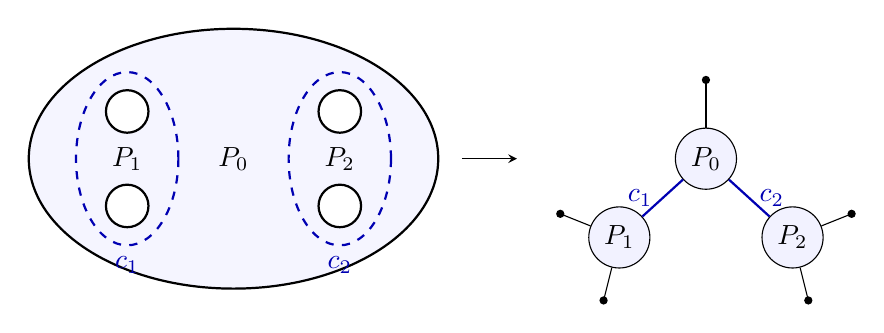
\begin{tikzpicture}[x=1cm,y=1cm,>=stealth]
	\draw[thick,fill=blue!4] (0,0) ellipse (2.6 and 1.65);
	\foreach \x in {-1.35,1.35}{
		\draw[thick,fill=white] (\x,0.6) circle (0.27);
		\draw[thick,fill=white] (\x,-0.6) circle (0.27);
		\draw[blue!70!black,thick,dashed] (\x,0) ellipse (0.65 and 1.1);
	}
	\node at (0,0) {\(P_0\)};
	\node at (-1.35,0) {\(P_1\)};
	\node at (1.35,0) {\(P_2\)};
	\node[blue!70!black] at (-1.35,-1.35) {\(c_1\)};
	\node[blue!70!black] at (1.35,-1.35) {\(c_2\)};
	\draw[->] (2.9,0)--(3.6,0);
	\begin{scope}[shift={(6,0)}]
		\node[circle,draw,fill=blue!5,inner sep=3pt] (p0) at (0,0) {\(P_0\)};
		\node[circle,draw,fill=blue!5,inner sep=3pt] (p1) at (-1.1,-1) {\(P_1\)};
		\node[circle,draw,fill=blue!5,inner sep=3pt] (p2) at (1.1,-1) {\(P_2\)};
		\draw[blue!70!black,thick] (p0)--node[left] {\(c_1\)}(p1);
		\draw[blue!70!black,thick] (p0)--node[right] {\(c_2\)}(p2);
		\draw (p0)--(0,1);
		\draw (p1)--(-1.85,-0.7);
		\draw (p1)--(-1.3,-1.8);
		\draw (p2)--(1.85,-0.7);
		\draw (p2)--(1.3,-1.8);
		\foreach \x/\y in {0/1,-1.85/-0.7,-1.3/-1.8,1.85/-0.7,1.3/-1.8}{
			\fill (\x,\y) circle (1.5pt);
		}
	\end{scope}
\end{tikzpicture}

	\caption[五边界球面的裤分解]{从五边界球面依次切下两条裤子，最后留下第三条。右图记录三个裤形分支的邻接关系：两个内部接缝各对应一条切割曲线，五个外端分别对应原来的五条边界。图记录拓扑粘合，不预设长度或角度。}
	\label{g1:fig:pants-tree}
\end{figure}

例如，闭的亏格 \(2\) 曲面需要 \(3\) 条切口，得到 \(2\) 条裤子；一次穿孔环面需要 \(1\) 条切口，得到 \(1\) 条裤子；五边界球面需要 \(2\) 条切口，得到 \(3\) 条裤子，如\cref{g1:fig:pants-tree}。恢复原曲面时，同一条裤子的两条边界可以彼此粘合，切口两侧因而可能属于同一块裤形曲面。

\ProseParagraphBreak

条件 \(\chi<0\) 来自每块裤形曲面的负 Euler 示性数。球面、圆盘、环带和闭环面分别有 Euler 示性数 \(2,1,0,0\)，沿闭曲线切开仍保持该数，因而不可能变成非空的裤形曲面之并。闭环面可以沿一条经线切成环带，但环带不是裤子。另一方面，裤形曲面本身满足 \(\chi=-1\)，其分解使用 \(0\) 条切口，符合公式，给出允许空曲线组的基本例子。

\ProseParagraphBreak

裤分解为后面的双曲几何提供了一个清楚的粘合问题：先给每条裤子配置适当的几何结构，再把对应边界按相容的数据接回去。拓扑分解记录块数与连接圆周；选定双曲几何结构后，边界长度与粘合扭转才成为新的数据。双曲裤子的存在与唯一性、边界长度的作用以及粘合中的扭转参数，都需要后卷的度量与测地线理论。这里已经确定的是分成多少块、沿哪些圆周连接，以及这些切口怎样反映曲面的亏格和边界。
% 纲要条目排为编号小节标题，并进入目录与 PDF 书签；说明段仍保留于纲要注释中。
